\documentclass[a4paper,twoside,phd]{BYUPhys}
% The BYUPhys class is for producing theses and dissertations
% in the BYU Department of Physics and Astronomy.  You can supply
% the following optional arguments in the square brackets to
% specify the thesis type:
%
%   senior  : Produces the senior thesis preliminary pages (default)
%   honors  : Produces the honors thesis preliminary pages
%   masters : Produces the masters thesis preliminary pages
%   phd     : Produces the PhD dissertation preliminary pages
%
% The default format is appropriate for printing, with blank pages
% inserted after the preliminary pages in twoside mode so you can
% send it directly to a two-sided printer. However, for ETD
% submission the blank pages need to be removed from the final output.
% The following option does this for you:
%
%   etd     : Produces a copy with no blank pages in the preliminary section.
%             Remove this option to produce a version with blank pages inserted
%             for easy double sided printing.
%
% The rest of the class options are the same as the regular book class.
% A few to remember:
%
%   oneside : Produces single sided print layout (recommended for theses less than 50 pages)
%   twoside : Produces double sided print layout (the default if you remove oneside)
%
% The BYUPhys class provides the following macros:
%
%   \makepreliminarypages : Makes the preliminary pages
%   \clearemptydoublepage : same as \cleardoublepage but doesn't put page numbers
%                           on blank intervening pages
%   \singlespace          : switch to single spaced lines
%   \doublespace          : switch to double spaced lines
%
% --------------------------- Load Packages ---------------------------------

% The graphicx package allows the inclusion of figures.  Plain LaTeX and
% pdfLaTeX handle graphics differently. The following code checks which one
% you are compiling with, and switches the graphicx package options accordingly.
\usepackage{ifpdf}
\ifpdf
  \usepackage[pdftex]{graphicx}
\else
  \usepackage[dvips]{graphicx}
\fi

%%%%%%%%%%%%%%%%%%%%%%%%%%%%%%%%%%%%%%%%%%%%%%%%%%%%%%%%%%%%%%%%%%
% Edited : Beeshanga
%
% If you need to include any code in the text use this package
% \usepackage{listings}
% It can be used to make key words bold, add colours, etc. Refer
% to http://en.wikibooks.org/wiki/LaTeX/Packages/Listings for
% more information.
%
% For theorems, propositions, proofs and assumtions use this
% package
% \usepackage{amsthm}
% For more information refer to the following website
% http://en.wikibooks.org/wiki/LaTeX/Theorems
%
%%%%%%%%%%%%%%%%%%%%%%%%%%%%%%%%%%%%%%%%%%%%%%%%%%%%%%%%%%%%%%%%%%

% The fancyhdr package allows you to easily customize the page header.
% The settings below produce a nice, well separated header.
\usepackage{fancyhdr}
  \fancyhead{}
  \fancyhead[LO]{\slshape \rightmark}
  \fancyhead[RO,LE]{\textbf{\thepage}}
  \fancyhead[RE]{\slshape \leftmark}
  \fancyfoot{}
  \pagestyle{fancy}
  \renewcommand{\chaptermark}[1]{\markboth{\chaptername \ \thechapter. #1}{}}
  \renewcommand{\sectionmark}[1]{\markright{\thesection \ #1}}


% The cite package cleans up the way citations are handled.  For example, it
% changes the citation [1,2,3,6,7,8,9,10,11] into [1-3,6-11].  If your advisor
% wants superscript citations, use the overcite package instead of the cite package.
\usepackage{cite}
\setlength{\parskip}{1em}

% The makeidx package makes your index for you.  To make an index entry,
% go to the place in the book that should be referenced and type
%  \index{key}
% An index entry labeled "key" (or whatever you type) will then
% be included and point to the correct page.
%\usepackage{makeidx}
%\makeindex

% The url package allows for the nice typesetting of URLs.  Since URLs are often
% long with no spaces, they mess up line wrapping.  The command \url{http://www.physics.byu.edu}
% allows LaTeX to break the url across lines at appropriate places: e.g. http://www.
% physics.byu.edu.  This is helpful if you reference web pages.
\usepackage{url}
\urlstyle{rm}

% If you have a lot of equations, you might be interested in the amstex package.
% It defines a number of environments and macros that are helpful for mathematics.
% We don't do much math in this example, so we haven't used amstex here.
\usepackage{amsmath}
\usepackage{amssymb}
\usepackage{subfigure}
\usepackage{cite}
\usepackage{amsxtra}
\usepackage{amsfonts}
\usepackage{graphicx}
\usepackage{multirow} % This is package for multi-rows in tables added on 7th July 2009 by Arif
%\usepackage{setspace}

% The caption package allows us to change the formatting of figure captions.
% The commands here change to the suggested caption format: single spaced and a bold tag
\usepackage[labelfont=bf,labelsep=colon]{caption}%[2008/04/01]
 \DeclareCaptionFormat{suggested}{\singlespace#1#2#3\par\doublespace}
 \captionsetup{format=suggested}


\usepackage{array}
\usepackage{multirow}
\usepackage{verbatim}
\usepackage{enumerate}

% Defining the symbols




% The hyperref package provides automatic linking and bookmarking for the table
% of contents, index, equation references, and figure references.  It must be
% included for the BYU Physics class to make a properly functioning electronic
% thesis.  It should be the last package loaded if possible.
%
% To include a link in your pdf use \href{URL}{Text to be displayed}.  If your
% display text is the URL, you probably should use the \url{} command discussed
% above.
%
% To add a bookmark in the pdf you can use \pdfbookmark.  You can look up its usage
% in the hyperref package documentation
\usepackage[bookmarksnumbered,pdfpagelabels=true,plainpages=false,colorlinks=true,
            linkcolor=black,citecolor=red,urlcolor=blue]{hyperref}

% ------------------------- Fill in these fields for the preliminary pages ----------------------------
%
% For Senior and honors this is the year and month that you submit the thesis
% For Masters and PhD, this is your graduation date
  \Year{2018}
  \Month{November 09,}
  \Author{Abhishek Satpathy}

% If you have a long title, split it between two lines. The \TitleBottom field defines the second line
% A two line title should be an "inverted pyramid" with the top line longer than the bottom.
  \TitleTop{Smart Contract Communication among Blockchains}
  %\TitleBottom{Line 2 of the Tile} % edited Beeshanga
 \DegreeTitle{Bachelor of Engineering
 \\ Software Engineering Stream} % edited Beeshanga

% Your research advisor
 \Advisor{Supervisor: Michael Johnson}

% The department undergraduate research coordinator
%  \UgradCoord{A}

% The representative of the department who will approve your thesis (usually the chair)
%  \DepRep{B}

% Acknowledge those who helped and supported you

  \Acknowledgments{
  \vspace{-1.5cm}
    \noindent I would like to acknowledge my supervisor Prof. Michael Johnson who has always been a great help throughout my degree and not just the thesis. Michael accepted to supervise my project proposal even though it was not related to one of his areas of research. 
    
    
    \noindent I would also like to acknowledge Mr. Kris Crnomarkovic who has been really helpful with long and tiring discussions about certain difficult issues that I during research. Kris's involvement with my theses is really appreciated.

  }


% The title of the department representative
%  \DepRepTitle{Chair}
  \Statement{
    \noindent I, Abhishek Satpathy, declare that this report, submitted as part of the requirement for the award of Bachelor of Engineering in the School of Engineering, Macquarie University, is entirely my own work unless otherwise referenced or acknowledged. This document has not been submitted for qualification or assessment at any other academic institution.
    \vspace{0.5cm}

    \noindent     Student's Name: Abhishek Satpathy

    \vspace{0.25cm}

    \noindent Student's Signature: Abhishek Satpathy

    \vspace{0.25cm}

    \noindent     Date: \today
    }

% The text of your abstract
\Abstract{
\vspace{-1.5 cm}
Blockchain technology has potential applicability in finance, supply-chain management, asset-tracking, web decentralization. Scalability and interoperbility are two major problems, hindering the applicability of blockchains in large-scale commercial architectures. Here, we discuss the application of a novel protocol that aims to solve the issues of scalability and interoperability of blockchains using a communication layer between multiple homogenous blockchains.
}



% Statement of Candidate



\fussy

\begin{document}

 % Start page counting in roman numerals
 \frontmatter

 %This command makes the formal preliminary pages.
 % You can comment it out during the drafting process if you want to save paper.

 \makepreliminarypages


%\clearemptydoublepage
\doublespace
%\include{Publications/publications}

% \clearemptydoublepage
%\include{Organization/organization}

 \clearemptydoublepage
\singlespace
 % Make the table of contents.
 \tableofcontents

\clearemptydoublepage
% Make the list of figures
\listoffigures

\clearemptydoublepage
% Make the list of tables
\listoftables

\clearemptydoublepage

% Start regular page counting at page 1
\mainmatter
%
\chapter{Introduction}
\label{chap:Introduction}
Blockchain technology has demonstrated enormous potential utility in multiple fields including "Internet of things", governance, finance, asset-tracking and web decentralization. 
 Scalability and interoperability are major problems, hindering the mainstream adoption of blockchains into these different fields of application. Current real-world blockchain implementations are practically limited to around 30 transactions per second. This issue arises from the current synchronous consensus mechanisms which require a wide time margin to ensure safety of the transactions. The demand for higher transaction throughput is rapidly increasing with the growing user base. One of the numerous ways of addressing this scalability problem is facilitating intercommunication among smart contracts on multiple separate blockchains. Prior to evaluating the problem of scalability, it is important to get familiar with some basics and terminology related to distrubuted ledgers and blockchains specifically.


\section{Hash Function}
A hash function is a one way mathematical construct that takes a data input of arbitrary length and outputs arbitrary data of a fixed length. The primary use of hashing in cryptography is maintaining the integrity of messages.Hashes are used in a blockchain to ensure the integrity of the data stored in each block.
\section{Public Key Cryptography}
Public key cryptography is extensively used on the blockchain. Accounts are essentially just public keys with an associated private key. The transactions are directly referenced to a particular public key. Anyone in possesion of the private key has the ability to initiate transactions on behalf the respective public key. The type of public key interface used on the most popular public blockchains is a called elliptic curve cryptography (ECC).
\section{Consensus}
Consensus is a mechanism which ensures that every node on the blockchain network is has the same exact copy of the data. A consensus mechanism syncs data across all nodes as and when those nodes connect to the network. Proof of work is by far the most popular consensus mechanism used in mainstream public blockchains. 
\section{Clients}
A client of the blockchain is the end-user software that ensures the blockchain synchronisation, generates and stores private keys, and facilitates transactions on behalf of the private key. 
\section{Transactions}
A transaction is a the transfer of a signed data package on the blockchain. It is a record of a computational activity that has taken place on the ledger. Any information that is stored and can retrieved is the result of a transaction. EVM transactions involve transfer of value. 
\section{Smart Contracts}
Smart Contracts are agents that facilitate the negotiation of a transaction on the blockchain without the use of another third party agent.

\section{Accounts}
Account on a blockchain is the hashed output of the public key associated with a transaction or a group of transactions referenced in the ledger.

\chapter{Background and Related Work}

\section{Project Goal}
The project title is quite broad and can be applied to a lot of different blockchains and other distributed ledger technologies that have smart contract functionality. Some of these possible blockchains are Ethereum, Hyperledger Fabric, Hyperledger Sawtooth, Cosmos, etc. However, in order to keep the scope of this project specific and achievable, the project is going to be focused on developing such a seamless smart contract communication protocol on multiple Ethereum private networks. Developing, a generic protocol such as TCP/IP for smart contract communication would be the ideal outcome but might turn out to be a daunting task for a project that has a time scope of about 15 weeks. \par
\par
Therefore, in order to keep the scope of the project specific and achievable, the project would aim to create a protocol for communicating messages across smart contracts on multiple Ethereum private networks. However, creating a generic protocol is still on the table, and if the timeline of the project permits then, a large amount of work will be put into delivering a generic protocol for platform-independent communication among smart contracts on multiple blockchains, such as Ethereum, Hyperledger Fabric, Hyperledger Sawtooth, or any other blockchain platform that has a Virtual machine and smart contract capability. \par
The questions that would need to be addressed in this thesis as deliverables would be the following:
\begin{itemize}
 

    \item• What is a secure way to encrypt a message so that it could be sent out of the blockchain without being subject to a man-in-the-middle attack?
    \item• How can the multiple blockchains achieve consensus of data?
    \item• How can a relay blockchain be secure without being the single point of failure?
    \item• How much information is needed to be communicated among the smart contract suites
of different blockchains?
    \item• What is best approach to make sure that the security of the information is not
compromised during communication?
    \item• What will be the improvement in the transaction throughput, once the technology is
implemented?
    \item• How can this technology be leveraged to solve the issue of scalability facing
blockchains today?
    \item• How will this technology be commercialized or made public for the greater good?
\end{itemize}

The deliverables for this particular project will be a suite of smart contract accounts on different blockchains that can communicate among each other using messages. The first stage will not include any transactions exchanged between the smart contracts as this exponentially increases the complexity and vulnerability of the application and might be extremely difficult to achieve within the critical time frame of the project. A transaction being defined as a message sent across by an externally owned account [6]. However, it is believed that further work can be done on the protocol to extend it to include financial transactions without compromising on security. Another deliverable for the project is an app built on react-native that can demonstrate this said smart contract communication functionality. The app will show all the different blockchains that it has been connected to, along with all the deployed smart contracts on the respective blockchains. The users of the app will be able to send messages across between any two smart contracts and be able to view the communication in almost real time.

\label{chap:LitReview}



\section{Related Projects \label{sec:CapResultsReview}}
Blockchain research as it has been mentioned already has been very limited in the past few years and has been mostly non-academic research done by independent organizations. Moreover, the technology is extremely nascent as the blockchain revolution was kicked off by bitcoins which have been around only for the last decade. This is a very short period for academic research to become mainstream in the field. However, some research has been done by non-academic organizations which is going to be the basis of all literature review. The research work done in this thesis will be built on top of that research. The following few research works lay the underlying framework for the research thesis on inter-blockchain communication, as described in this thesis project. Most of the following research is non- academic and therefore the availability of good quality documentation is sparse. However, best efforts have been put into understanding those previous works and, more importantly, it has been made sure that those works are very accurately described in this paper.


\subsubsection{BTC Relay}
BTC Relay is a bridge between the bitcoin blockchain and Ethereum smart contracts. It allows smart contracts on the Ethereum blockchain to securely verify bitcoin transactions. BTC Relay is an Ethereum Smart Contract that stores bitcoin block headers. These block headers are then used to build a lighter version of the bitcoin blockchain with enough data just to verify the validity of all the transactions. The bitcoin blockchain headers are sent to the BTC Relay smart contracts. These headers are then used to verify the validity of the transactions. This approach does not use a relay chain. It is also not a very scalable solution as it does not allow a two-way communication link between the blockchains. The entire light-weight version of the bitcoin blockchain has to be built from the block headers which is a computing resource intensive task and therefore might not be extremely viable for large scale use cases and connectivity across multiple blockchains. However, BTC Relay is a good starting point for reviewing attempts that have already been made in this field. [8]
\subsubsection{Peace Relay}
Peace Relay is very similar technology to BTC Relay. However, it is built for a different purpose of connecting two different Ethereum blockchains i.e. Ethereum and Ethereum Classic. Peace Relay works both ways between Ethereum Classic and Ethereum and vice-versa. Similar to BTC Relay, the Merkle Patricia headers are sent to the smart contract on the receiver blockchain that stores all the headers and verifies whether the header is valid before adding it
to the light-weight chain. The contract then allows the submission of Merkle proofs by users in order to verify the validity of the transactions [9]. \par
In order to send transactions from one blockchain to the other, Peace Relay uses locking contracts which peg the amount being transferred from the sender blockchain and then generate the same number of tokens on the receiving blockchain, using a corresponding smart contract. This process is very unscalable just like BTC Relay, and the contract execution can become exponentially complex with the addition of more blockchains in the relay. However, this demonstrates that a possible communication between two Ethereum blockchains is definitely possible. There is definitely a more effective and scalable solution which can achieve the same effect. Finding that more effective and scalable solution is the main objective of this research paper.
\subsubsection{Cosmos: Inter-Blockchain Communication Protocol}
Cosmos is a network connecting multiple independent blockchains. Cosmos has a main network which acts very much like a connector chain, called the Cosmos Hub. All the other blockchains connected to the Cosmos Hub are called Zones. A Cosmos zone is a separate, independent blockchain that uses the main blockchain, which is the Hub, for achieving global consensus on the network. Cosmos uses the protocol called Inter-blockchain Communication (IBC) for connectivity between the hub and all the zones. IBC uses data packets to send information across between the zones and the hub. There are two types of transactions in the IBC protocol; an IBCBlockCommitTx transaction and an IBCPacketTx transaction. The first kind of transaction allows a zone to prove to any observer of its most recent block-hash. The latter kind of transaction allows a blockchain to prove to any observer that the given packet was indeed published by the sender's application, via a Merkle-proof to the recent block-hash. The Cosmos Hub can also be used as a bridge between different blockchains such as any Bitcoin or Ethereum blockchain. The transaction throughput of the Cosmos blockchains is currently unknown, however, the zones use a Tendermint core which uses a Byzantine Fault Tolerant consensus mechanism and claims a transaction throughput of about 10000 transactions per second. [10] \par
Cosmos’s IBC currently seems to be the most promising background work, on which the entire research work of this project could be built upon. If this research project is successful, then this could most likely be work done on top of Cosmos IBC.
\subsubsection{Interledger}
Interledger is an open suite of protocols for connecting all types of ledgers and payment systems. Interledger uses connectors to route payments across different blockchains. In order to connect the blockchains, Interledger uses a transport protocol called STREAM, which is a multiplexed system for transporting money and data across blockchains connected via the Interledger protocol. It essentially uses multiple streams of data over the Interledger Protocol (ILP). A stream is a logical, bi-directional channel of ordered bytes and money within a STREAM connection. STREAM is a generic transport protocol for different ledgers which is a generic protocol, such as TLS on the internet. [13] [14] \par
However, STREAM on the Interledger Protocol is designed specifically for currency transactions and payments blockchains in mind. If, however, work could be done on this protocol to develop a generic blockchain communication protocol for executing all sorts of transactions and not just payments and data, then that would be the ideal outcome of this research project. \par
All the literature review mentioned above might not end up being the background work for this project. However, these lay a solid foundation for the ways in which the ideal outcome for this research project could be accomplished. More importantly, these show the different approaches taken by different parties working on this problem, that did not have a very optimal outcome and, therefore, such paths could be avoided. Furthermore, these background research works provide this research project a direction which would most likely lead towards the ideal outcome.

\chapter{Literature Review}
\label{chap:singleuser}

\section{Polkadot Framework \label{sec:Intro-ChapUserSelec}}
Polkadot is a protocol that facilitates the exchange information across independent blockchain networks. It aims to solve the same issues that this paper examining in detail. Polkadot is a good framework to build upon. It is a scalable heterogenous multi-chain that used data structures called heterogenous parachains or parallelised chains. There are multiple concepts that need to be familiarised before diving deeper into the architecture of a heterogenous parachain. The concept are discussed in the section below.

\section{Validators}
Validators are nodes on the relay-chain in charge of making new blocks visible to the network. 
\section{Nominators}
Nominators are nodes that are stake-holding parties which contrubute to the bond contributed by the validator. Teamed up with collator nodes nominators resemble the miners in the current blockchain architecture.
\section{Collators}
Collator nodes assist validator nodes in producing valid parachain blocks. These nodes bundle all the transactions into blocks and pass them onto validators, to be validated using zero-knowledge proofs.
\section{Fishermen}
Fisherman nodes are the gatekeepers of the polkadot network. They hunt for bounty incase of any illicit activy on the network such as a stolen security key.

\section{Heterogenous Multichain Architecture \label{sect:RelWorksingle-user}}

\chapter{Experimental Approaches}
\label{chap:Homogenous Multichain Architecture}


\section{Mirrored Smart Contracts}
The methodology and approach will be to create a messaging protocol that can be used in order for smart contracts to communicate among different Ethereum blockchains. The rough sketch of the protocol has been demonstrated in the figure 1.

\begin{figure}[t]
\centering
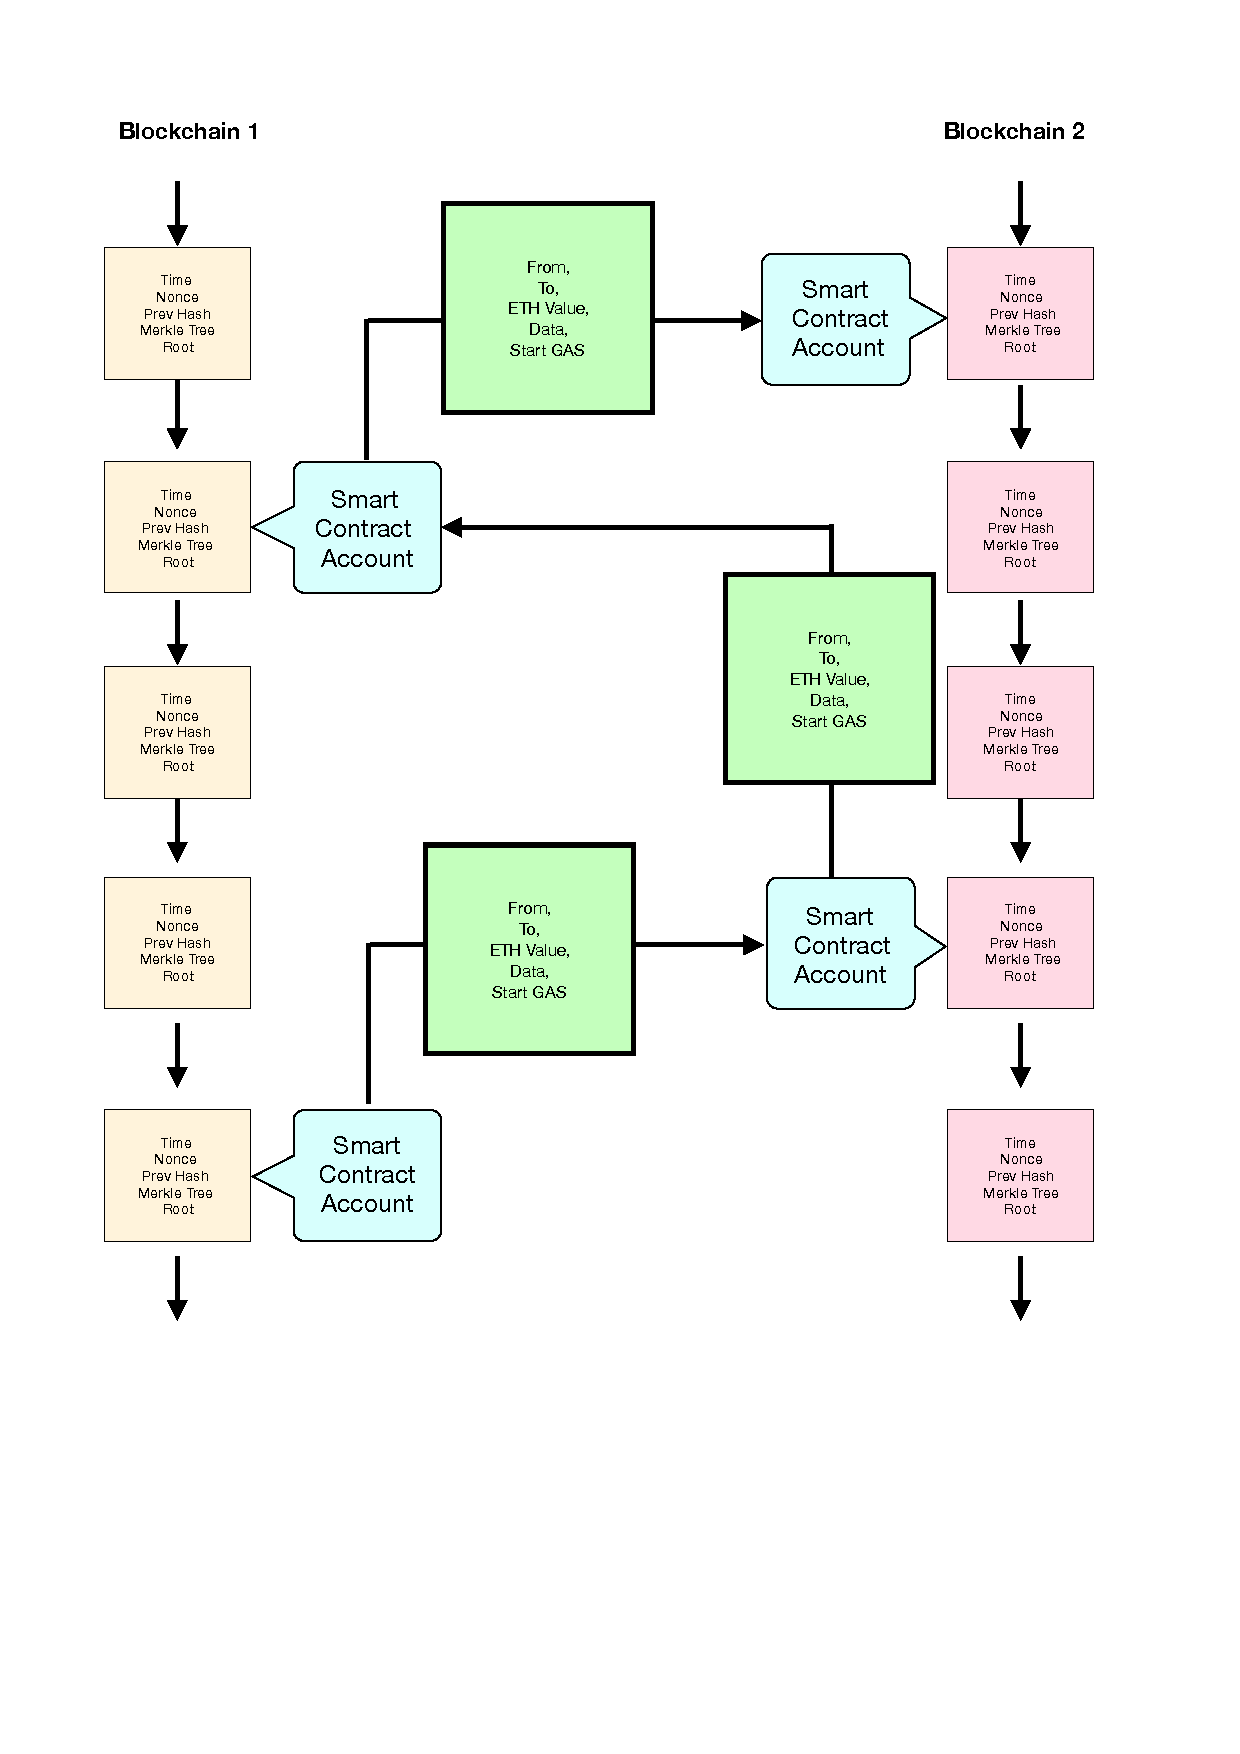
\includegraphics[width=8cm]{cap1}
\caption{Smart contract accounts sending messages across blockchains.}
\label{fig:cap1}
\end{figure}

\section{Relay Chain}
The approach to solve the issue of adresss collision that is ineveitable in the previous approach will be to create a relay chain that stores the unique blockchain addresses of each homogenous chain on the relay chain. Each separate blockchain will therefore have a separate unique address on the relay chain. The messages that are being transmitted between the smart contract will hence contain a from address which will be generated using a combination of the chain address on the relay chain and the smart contract account address. The address generation function will have to be researched and appropriately tested in order to avoid errors and collisions. This approach should be appropriate to achieve the task at hand.
\section{Sharding}
\label{sec:ConclusionsConclusions}

\clearemptydoublepage
\chapter{Experimental Results}
\chapter{Protocol Architecture}
\chapter{Conclusion}
\chapter{Further Improvements}
\chapter{Glossary}
\chapter{Acronyms}
\label{chap:abbreviations}

\begin{tabbing}

ADDR \qquad \qquad \= Account Address\\
ASIC \qquad \qquad \= Application Specific Integrated Circuit\\
BFT \> Byzantine Fault Tolerance/Tolerant\\
BTC \> Bitcoins\\
DAO \> Decentralized Autonomous Organization\\
dApp \> Decentralized Application\\
DDoS \> Distributed Denial of Service\\
ETH \> Ethereum\\
EVM \> Ethereum Virtual Machine\\
multisig \> Multiple-Signatures\\
P2P \> Peer to peer\\
PKI \>Public Key Interface\\
PoA \> Proof of Authority\\
PoW \> Proof of Work\\
PoS \> Proof of Stake\\
SHA \> Secure Hashing Algorithm\\
\end{tabbing}


%\phantomsection \addcontentsline{toc}{chapter}{Index}
% \renewcommand{\baselinestretch}{1} \small \normalsize
% \printindex

\appendix
\chapter{Revised Project Plan}
\section{Abstract}
Blockchain scalability is one of the major problems that need to be addressed in the entire blockchain space. Of the many approaches for scaling blockchains, facilitating intercommunication of smart contracts among multiple blockchains while maintaining consensus is a promising approach. This paper lays the project road map for the research regarding a novel protocol for intercommunication among multiple private Ethereum blockchains. The paper also discusses how this protocol can be demonstrated using an app built on react-native that could interface with the blockchains and help facilitate and demonstrate this interconnectivity protocol. Moreover, the paper provides a detailed project plan along with background and literature review, approach and methodology, intended research outcome, and expected impact of the outcome.
\section{Introduction and Background}
Blockchains have an immense potential to revolutionize the way the internet is being used today. Blockchain and Distributed ledger technology will lead the way into what is being termed as Web 3.0 [1], in which there is no point of central control like Google, etc., and in which data is owned by the peers and not the big data firms. Until now, blockchains and distributed ledger technology have only been synonymous with Bitcoins and other cryptocurrencies. However, this new technology has numerous potential applications in many different fields such as supply chain management, distributed computing, and many other applications that still need to be discovered. \par
Blockchains available at the moment are far away from being massively scalable in order to cater for these potential applications on a global scale. With an average of about 15 transactions per second [2], popular blockchains like Ethereum are far from being scalable. Numerous attempts have been made in order to scale blockchains and improve the transaction rates. Just in comparison with other payment platforms such as VISA and Mastercard, VISA does on average 1667 transactions per second with a peak capacity of about 56000 transactions per second [3]. Similarly, Mastercard processes about 2834 transactions per second on average and has a peak operating capacity of about 95000 transactions per second [4]. However, it is important to note that VISA and Mastercard are platforms meant only for payments processing. A public blockchain such as Ethereum can run DApps. DApps are distributed applications that can run on the EVM, the Ethereum Virtual Machine, which is a giant virtual computer that gathers its computing resources from all the computers running on the Ethereum Public Network. Each DApp is essentially a suite of smart contracts that work together to achieve the functionality of the DApp in a completely decentralized and peer-to-peer network [5]. Smart Contracts are autonomous agents on the blockchain that execute a transaction when certain conditions are met [6]. Each request on a DApp is executed as a smart contract transaction on the blockchain. As of writing this, the Ethereum public blockchain has 1657 decentralized apps and the number is rapidly increasing every day. With a transaction rate of about 15 transactions per second, this creates a serious bottleneck on the blockchain for running transactions. \par
A blockchain or a distributed ledger is a secure mechanism to run these transactions and sync the data across all the nodes in the network in order to make it secure and tamper proof. This same mechanism that makes blockchains, primarily so secure also make them massive unscalable and slow. There are many ways in which this problem of transaction scalability of blockchains can be solved. One of the solutions is to enable facilitation of smart contracts to be able to communicate among themselves while running on separate blockchains. Thus, each DApp could run on its own separate blockchain while communicating with smart contracts on multiple blockchains to achieve consensus of data, consensus being the main factor that makes blockchains tamper resistant. This project is going to explore possible solutions to this smart contract communication problem among separate blockchains, in a fast and secure way, so as to maintain the fault tolerance capability that these blockchains exhibit.

\section{Project Scope and Deliverables}
The project title is quite broad and can be applied to a lot of different blockchains and other distributed ledger technologies that have smart contract functionality. Some of these possible blockchains are Ethereum, Hyperledger Fabric, Hyperledger Sawtooth, Cosmos, etc. However, in order to keep the scope of this project specific and achievable, the project is going to be focused on developing such a seamless smart contract communication protocol on multiple Ethereum private networks. Developing, a generic protocol such as TCP/IP for smart contract communication would be the ideal outcome but might turn out to be a daunting task for a project that has a time scope of about 15 weeks. \par
\par
Therefore, in order to keep the scope of the project specific and achievable, the project would aim to create a protocol for communicating messages across smart contracts on multiple Ethereum private networks. However, creating a generic protocol is still on the table, and if the timeline of the project permits then, a large amount of work will be put into delivering a generic protocol for platform-independent communication among smart contracts on multiple blockchains, such as Ethereum, Hyperledger Fabric, Hyperledger Sawtooth, or any other blockchain platform that has a Virtual machine and smart contract capability. \par
The questions that would need to be addressed in this thesis as deliverables would be the following:
\begin{itemize}
 

    \item• What is a secure way to encrypt a message so that it could be sent out of the blockchain without being subject to a man-in-the-middle attack?
    \item• How can the multiple blockchains achieve consensus of data?
    \item• How can a relay blockchain be secure without being the single point of failure?
    \item• How much information is needed to be communicated among the smart contract suites
of different blockchains?
    \item• What is best approach to make sure that the security of the information is not
compromised during communication?
    \item• What will be the improvement in the transaction throughput, once the technology is
implemented?
    \item• How can this technology be leveraged to solve the issue of scalability facing
blockchains today?
    \item• How will this technology be commercialized or made public for the greater good?
\end{itemize}

The deliverables for this particular project will be a suite of smart contract accounts on different blockchains that can communicate among each other using messages. The first stage will not include any transactions exchanged between the smart contracts as this exponentially increases the complexity and vulnerability of the application and might be extremely difficult to achieve within the critical time frame of the project. A transaction being defined as a message sent across by an externally owned account [6]. However, it is believed that further work can be done on the protocol to extend it to include financial transactions without compromising on security. Another deliverable for the project is an app built on react-native that can demonstrate this said smart contract communication functionality. The app will show all the different blockchains that it has been connected to, along with all the deployed smart contracts on the respective blockchains. The users of the app will be able to send messages across between any two smart contracts and be able to view the communication in almost real time.

\section{Literature Review}
Blockchain research as it has been mentioned already has been very limited in the past few years and has been mostly non-academic research done by independent organizations. Moreover, the technology is extremely nascent as the blockchain revolution was kicked off by bitcoins which have been around only for the last decade. This is a very short period for academic research to become mainstream in the field. However, some research has been done by non-academic organizations which is going to be the basis of all literature review. The research work done in this thesis will be built on top of that research. The following few research works lay the underlying framework for the research thesis on inter-blockchain communication, as described in this thesis project. Most of the following research is non- academic and therefore the availability of good quality documentation is sparse. However, best efforts have been put into understanding those previous works and, more importantly, it has been made sure that those works are very accurately described in this paper.
subsubsection{BTC Relay}
BTC Relay is a bridge between the bitcoin blockchain and Ethereum smart contracts. It allows smart contracts on the Ethereum blockchain to securely verify bitcoin transactions. BTC Relay is an Ethereum Smart Contract that stores bitcoin block headers. These block headers are then used to build a lighter version of the bitcoin blockchain with enough data just to verify the validity of all the transactions. The bitcoin blockchain headers are sent to the BTC Relay smart contracts. These headers are then used to verify the validity of the transactions. This approach does not use a relay chain. It is also not a very scalable solution as it does not allow a two-way communication link between the blockchains. The entire light-weight version of the bitcoin blockchain has to be built from the block headers which is a computing resource intensive task and therefore might not be extremely viable for large scale use cases and connectivity across multiple blockchains. However, BTC Relay is a good starting point for reviewing attempts that have already been made in this field. [8]
\subsubsection{Peace Relay}
Peace Relay is very similar technology to BTC Relay. However, it is built for a different purpose of connecting two different Ethereum blockchains i.e. Ethereum and Ethereum Classic. Peace Relay works both ways between Ethereum Classic and Ethereum and vice-versa. Similar to BTC Relay, the Merkle Patricia headers are sent to the smart contract on the receiver blockchain that stores all the headers and verifies whether the header is valid before adding it
to the light-weight chain. The contract then allows the submission of Merkle proofs by users in order to verify the validity of the transactions [9]. \par
In order to send transactions from one blockchain to the other, Peace Relay uses locking contracts which peg the amount being transferred from the sender blockchain and then generate the same number of tokens on the receiving blockchain, using a corresponding smart contract. This process is very unscalable just like BTC Relay, and the contract execution can become exponentially complex with the addition of more blockchains in the relay. However, this demonstrates that a possible communication between two Ethereum blockchains is definitely possible. There is definitely a more effective and scalable solution which can achieve the same effect. Finding that more effective and scalable solution is the main objective of this research paper.
\subsubsection{Cosmos: Inter-Blockchain Communication Protocol}
Cosmos is a network connecting multiple independent blockchains. Cosmos has a main network which acts very much like a connector chain, called the Cosmos Hub. All the other blockchains connected to the Cosmos Hub are called Zones. A Cosmos zone is a separate, independent blockchain that uses the main blockchain, which is the Hub, for achieving global consensus on the network. Cosmos uses the protocol called Inter-blockchain Communication (IBC) for connectivity between the hub and all the zones. IBC uses data packets to send information across between the zones and the hub. There are two types of transactions in the IBC protocol; an IBCBlockCommitTx transaction and an IBCPacketTx transaction. The first kind of transaction allows a zone to prove to any observer of its most recent block-hash. The latter kind of transaction allows a blockchain to prove to any observer that the given packet was indeed published by the sender's application, via a Merkle-proof to the recent block-hash. The Cosmos Hub can also be used as a bridge between different blockchains such as any Bitcoin or Ethereum blockchain. The transaction throughput of the Cosmos blockchains is currently unknown, however, the zones use a Tendermint core which uses a Byzantine Fault Tolerant consensus mechanism and claims a transaction throughput of about 10000 transactions per second. [10] \par
Cosmos’s IBC currently seems to be the most promising background work, on which the entire research work of this project could be built upon. If this research project is successful, then this could most likely be work done on top of Cosmos IBC.
\subsubsection{Interledger}
Interledger is an open suite of protocols for connecting all types of ledgers and payment systems. Interledger uses connectors to route payments across different blockchains. In order to connect the blockchains, Interledger uses a transport protocol called STREAM, which is a multiplexed system for transporting money and data across blockchains connected via the Interledger protocol. It essentially uses multiple streams of data over the Interledger Protocol (ILP). A stream is a logical, bi-directional channel of ordered bytes and money within a STREAM connection. STREAM is a generic transport protocol for different ledgers which is a generic protocol, such as TLS on the internet. [13] [14] \par
However, STREAM on the Interledger Protocol is designed specifically for currency transactions and payments blockchains in mind. If, however, work could be done on this protocol to develop a generic blockchain communication protocol for executing all sorts of transactions and not just payments and data, then that would be the ideal outcome of this research project. \par
All the literature review mentioned above might not end up being the background work for this project. However, these lay a solid foundation for the ways in which the ideal outcome for this research project could be accomplished. More importantly, these show the different approaches taken by different parties working on this problem, that did not have a very optimal outcome and, therefore, such paths could be avoided. Furthermore, these background research works provide this research project a direction which would most likely lead towards the ideal outcome.
\section{Approach and Methodology}
The approach towards the solution to the problem being discussed in this paper will be quite different from other academic research. The main reason behind this is that no peer-reviewed academic research work has been done already in the inter-blockchain communication space. That alone would be the biggest hurdle in conducting this project methodically. Due to the availability of inadequate documentation or complete lack of it, proper understanding of the existing work that has already been done in the area will be difficult. It has already been mentioned in the literature review section that the background research work done in this area is quite sparse. There is a need for new innovation, research and a completely novel approach and methodology.\par
The methodology and approach will be to create a messaging protocol that can be used in order for smart contracts to communicate among different Ethereum blockchains. The rough sketch of the protocol has been demonstrated in the figure 1. The diagram shows two blockchains, each with multiple smart contract accounts that are sending messages across to each other. The only issue in the current diagram is that there is no method to specify which blockchain the respective smart contract accounts belong to. The approach to solve this issue will be to create a relay chain which will store the unique blockchain addresses of each blockchain on the relay chain. Each separate blockchain will therefore have a separate unique address on the relay chain. The messages that are being transmitted between the smart contract will hence contain a from address which will be generated using a combination of the chain address on the relay chain and the smart contract account address. The address generation function will have to be researched and appropriately tested in order to avoid errors and collisions. This approach should be appropriate to achieve the task at hand.

\begin{figure}[t]
\centering
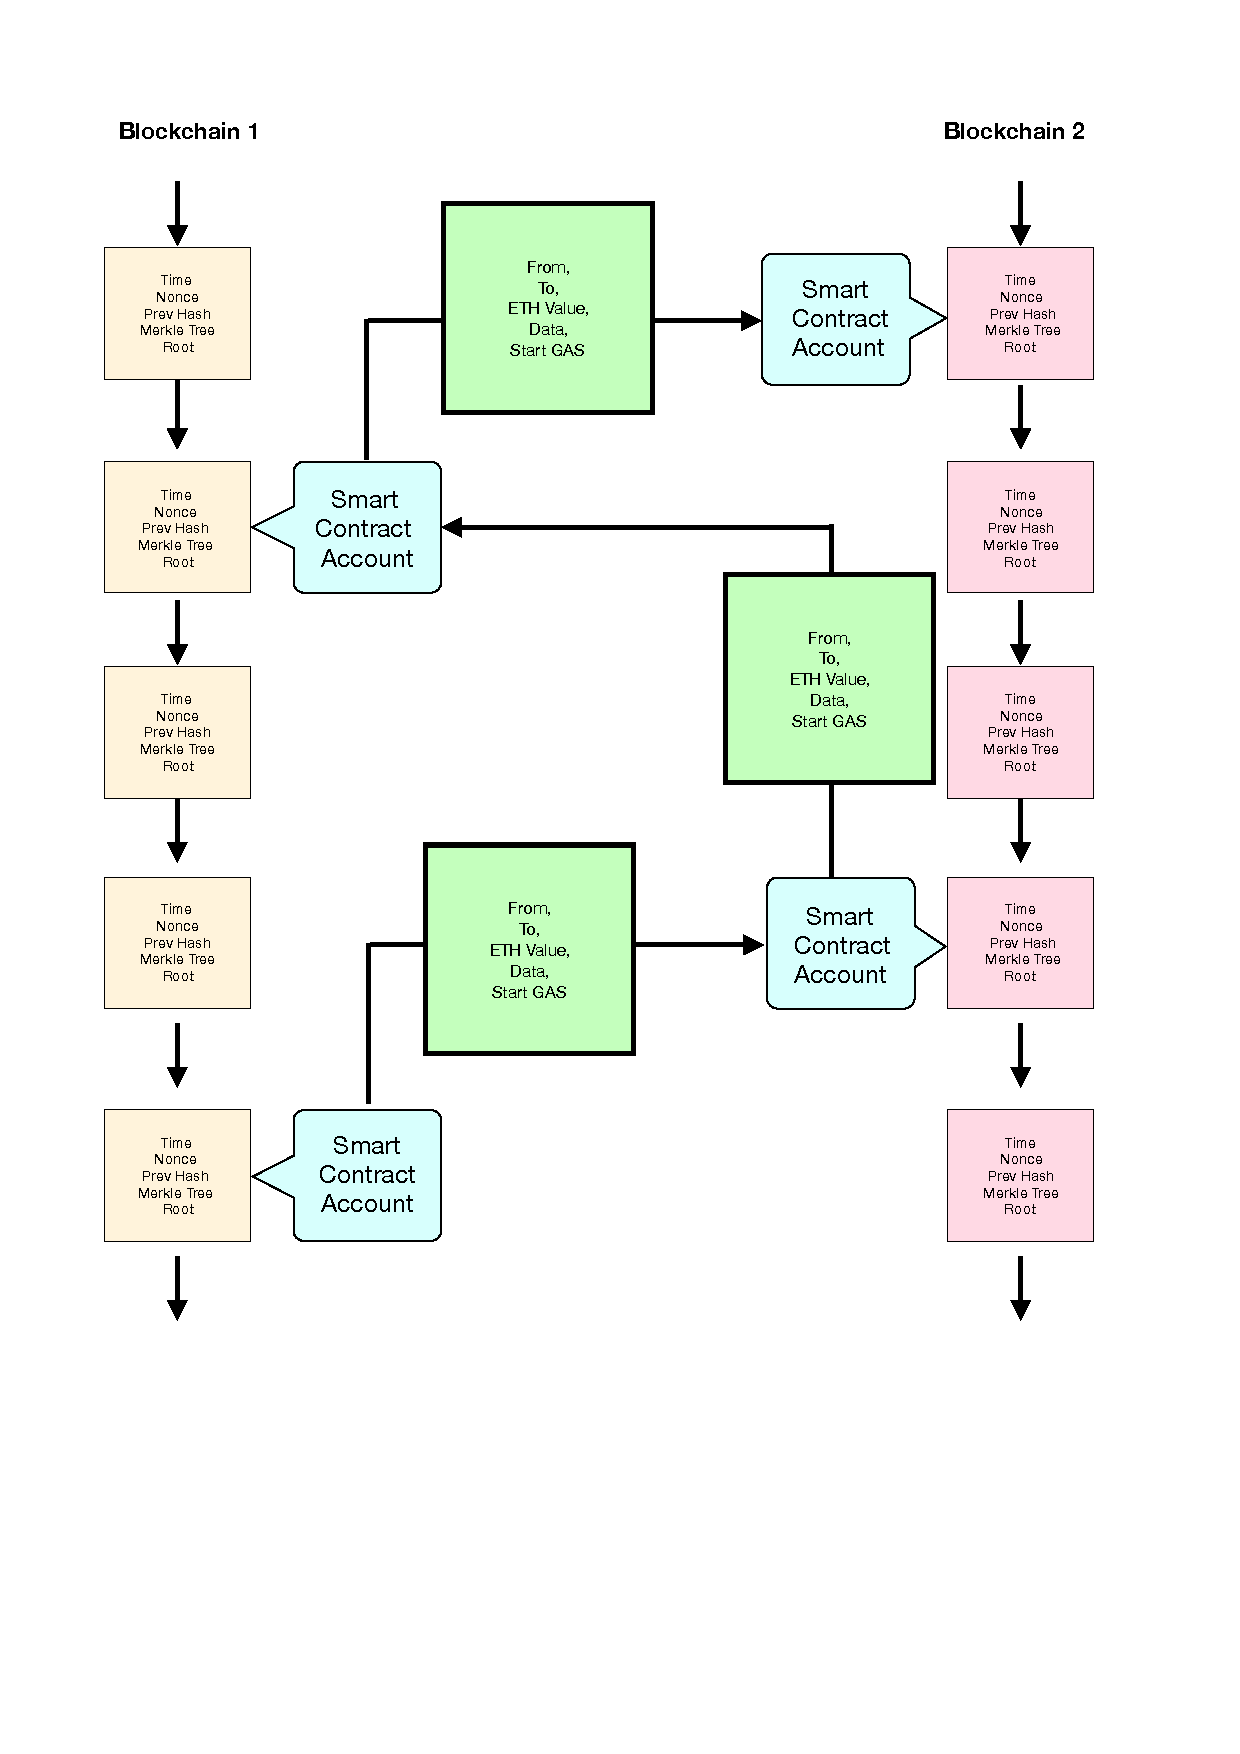
\includegraphics[width=8cm]{cap1}
\caption{Smart contract accounts sending messages across blockchains.}
\label{fig:cap1}
\end{figure}

\section{Project Timeline}
The thesis project has a very strict timeline and has to be completed within roughly the 15 weeks available in session 2 of 2018. The complete graphical representation of the project timeline has been provided in the GANTT chart attached in appendix I. The first stage of the project which is project planning and literature review has already been completed in this report. The other stages of the project have been described in detail in this section below. \par
The following provides the detailed timelines of all the tasks that have been identified in the GANTT chart in appendix I
\subsection{Project Planning and Literature Review}
\subsubsection{Study Available Research}
In this part of the project, existing research in the field
was studied in order to gain in depth knowledge of the field and get a good grasp of the main concepts around blockchain development. This part of the project roughly took 4 weeks to complete, beginning on 26th of February 2018.
\subsubsection{Find Suitable Background Work}
After studying the available research, work had to be done in order to segregate the research that can be used as a foundation to this particular thesis. All this suitable work has been discussed in the literature review section. This took about 3 weeks to complete.
\subsubsection{Develop a Timeline}
After the literature review a complete project timeline had to be developed, and all the specific breakdown of tasks and phases had to be identified. This part took roughly about 2 weeks to complete.
\subsubsection{Write a project plan}
The final part of this project planning stage was actually writing the project plan report for the thesis. This should have taken roughly 4 weeks, however due to exams and unexpected sickness it has taken so long to finish and will be submitted by 2nd July 2018.
\subsection{App Development and Blockchains Setup}
\subsubsection{Setup a React Native App}
The connectivity suite will have a front-end for
demonstration purposes. The front-end app will be built using react-native for both iOS and Android. This setup will take roughly about 2 weeks.
\subsubsection{Create two private Ethereum Networks}
The application protocol described in this paper will use these two networks to establish a connectivity suite among them securely. This task is effectively completed, as there are two blockchains already
running.
\subsubsection{Connect the Private networks to the app}
The blockchains will have to be
connected to the front-end app in order to demonstrate the connectivity of the two
different chains. This task will be done in roughly 1 week.
\subsubsection{Test the app and blockchain connectivity}
The connectivity between the app and
the blockchains has to be tested in order to proceed to the next phases of the project.
This will take about a week to test properly.
\subsection{Develop the Interconnectivity Protocol}
\subsubsection{Build an application to connect the blockchains}
The entire success of the thesis
relies on the successful implementation of this part alone. This connectivity protocol is the main feature of the project. Currently, it has been allocated 3 weeks of completion time, however, it might take more, and the timeline will be modified accordingly.
\subsubsection{Test the Application connectivity}
The connectivity protocol among different blockchains needs to be thoroughly tested for failures and corner cases, and therefore, a week of testing time has been given to this stage.
\subsubsection{Create a generic protocol from the app}
The paper discusses a protocol for communication among different blockchains and therefore a standard communication protocol that can be applied to multiple blockchains has to be developed, given there is enough time for successful completion. This stage has been allocated a time frame of about 3 weeks.
\subsubsection{Test the generic protocol}
The generic protocol for smart contract communication will have to be tested on multiple blockchains other than Ethereum for platform independence. The time allocated for this task is about 2 weeks.
\subsection{Writing the Thesis}
\subsubsection{Write the thesis}
The most important part of the thesis is definitely the thesis.
Writing the thesis will take a significant amount of time and therefore a time frame
of about 3 weeks has been allocated to this task.
\subsubsection{Spelling and grammar review}
The thesis will then be checked for any spelling
and grammar errors. This is really necessary as it is really easy to go off track with
grammar on a thesis of this size. The time allocated for this task is about 4 days.
\subsubsection{Proof Reading}
The thesis will then need to be proof read for coherence and ease of understanding of the concepts described. This task has been allocated about 5
days.
\subsection{Peer and Self Review}
\subsubsection{Self-review Thesis}
The thesis will be self-reviewed, and the references will be
cross checked before handing it over to the supervisor for suggestions and
comments. This task has been given a week for completion.
\subsubsection{Accommodate changes and suggestions}
The thesis will then be sent to the supervisor for
review and comments. Currently, a week’s time has been given to this task, however, this timeline might vary significantly depending on the availability of the supervisor for review. These changes will be appropriately accommodated in the timeline after further consultation with the supervisor.
\subsubsection{Accommodate changes and suggestions}
The supervisor will definitely have comments and suggestions which will need to be accommodated in the thesis before final submission. This task has been currently allocated about a week, however, the time line will vary depending on the amount of changes suggested by the supervisor. The project timeline will be modified based on the amount work that needs to be done.
\subsubsection{Final Submission}
The prospective final submission date for the thesis is set on 5th December 2018. However, this date will vary depending on the time taken for supervisor review and the amount of changes that need to be accommodated after the review. Therefore, the final date of submission might vary. Any changes to this date will be communicated with the supervisor in due time.

\section{Feasibility and Training}
The successful completion of this project relies on a lot of research and innovation. A lot of research has to be accomplished in the area of inter-blockchain communication and networking before a protocol for communication between smart contracts on multiple blockchains can be developed. Some of the successful or partly successful attempts at developing this technology have already been demonstrated in the literature review. Along with the research work available from the literature review, strong grasp of concepts in Networking such UDP, HTTPS, TLS, etc., is required for a successful completion of this thesis. More importantly, concepts in cyber security are extremely important as well. Blockchains heavily use Public Key Infrastructure (PKI); hashing algorithms such as SHA-256, ETH-Hash, etc.; Byzantine Fault Tolerance algorithms and many other mathematically complex algorithms and data structures. Thorough understanding of the above-mentioned algorithms and other consensus algorithms such as proof of work and proof of stake is also extremely necessary. \par
Ethereum blockchains use a data structure known as Merkle trees in order to store transaction information in the blocks. A thorough understanding of these Merkle tree data structures and Merkle tree headers is really necessary in order to communicate information effectively among blockchains to achieve consensus. Furthermore, a good understanding of the Cryptography and information security concepts taught in COMP343 is also very crucial. All the notes from COMP343 will have to be revised. All the cyber security threats such as DDoS, Man-in-the- middle attack, double spending attack and Sybil fault, etc., will have to be thoroughly reviewed.\par
The fully spec’d MacBook Pro which is available should be enough for the development of the app and running the Docker containers on Amazon Web Services (AWS) VM instances. However, if there is a possibility of access to a Linux computer or an iMac in one of the computer labs on campus, that would be a very helpful resource towards the project. \par
The university allows reimbursements of up to $400 for this thesis project. All of those $400 will be used towards running Docker containers on AWS VM instances for running the private blockchain nodes. The nodes will be running during testing and prototyping. The instances will be shut down during downtime in order to cut costs. Purchase of any hardware would not be necessary as there is an old iPhone at disposal which can be used for iOS testing purposes and there are multiple emulators available on Android studio for Android testing.

\section{Expected Outcomes and Impact}
The expected outcome of this project is to create a protocol which will allow multiple blockchain networks to send messages among themselves and communicate effectively, using this protocol. This will also include creating a consensus mechanism for all the blocks on the multiple blockchains to validate each other. The blockchains will all be connected to a react- native app which will, in turn, connected to the relay chain. The relay chain will act as a connector blockchain for all the blockchains that are functioning and communicating among themselves. This does seem like a very daunting task for a project that has a time-frame of about 15 weeks. However, if the outcome of the research project is two Ethereum blockchains with multiple smart contracts, all being able to communicate among themselves using the 160- bit addresses, then that would be considered as a positive outcome for the project. \par
The research project will have three definite outcomes. The first outcome is that the communication protocol among smart contracts on multiple blockchains in possible and successfully implemented. This would be the most ideal outcome and will have the greatest impact in terms of achievement. This could even lead to a fully commercialized technology that will have a massive impact on the entire blockchain industry. The second possible outcome would be that such a communication protocol as described in section 4 of this document is possible, however due to time and resource limitations, such a feat could not be achieved within the time frame of this thesis project. This outcome might not be ideal but leaves room for further development outside the scope of this research thesis and outside the 15 weeks of available time. However, this is still a very positive outcome and further research will be done to accomplish its full effect. The third and the most unwarranted outcome of this research project will be that such connectivity among smart contracts on different blockchains is not possible. This would not be ideal as this would invalidate all the attempts that have been taken so far in this space in order to improve the scalability of all blockchains. This outcome wouldimply that a completely different approach towards achieving scalability on blockchains has to be taken. Therefore, no matter what the final outcome of this research project is, it is going to revolutionize the way in which the issue of blockchain scalability is being dealt with. The impact of this project is going to be enormous on the entire blockchain ecosystem. \par
Blockchain technology has the potential to be beneficially applied to numerous different industries. It shows immense ability to disrupt industries like finance, supply chain, energy, software, distributed computing, among many other commercial use cases that are yet to be identified and harnessed. One of the main issues that will stop blockchains from becoming mainstream and going on to disrupt these industries is their ability to scale and handle the millions of transactions which are going to be flooding these blockchains once they are put to effective use. This research addresses the particular issue of scalability facing blockchains. If successful, this project could lead to blockchains becoming effective enough for mainstream use. This will, therefore, lead to complete transition of industries into the age of decentralized computing. It will impact the entire internet and the concept of trust on the internet. The entirely new form of trust on the internet based on mathematical proofs will lead to a new secure, decentralized internet. The impact of this project will be significant on many industries, will disrupt many other and even create a fresh few. The success of this project will be the foundation on which the entire framework of a completely secure and trustless Web 3.0 could be built.

\section{References}
As per the marking rubric, it is mentioned that 40\% of marks for this project plan are contributed from the in-depth review of appropriate peer-reviewed literature. However, due to the uniqueness and novelty of the project, no previous academic or peer-review work is available in this area of blockchain research. All the research and background work has been done by independent third-party organizations and startups. Some of the articles on Medium have also been used for references. The literature review might not be adequate enough due to lack of detailed academic research available. An academic paper even mentions that about 80\% of all academic research in the blockchain space has been done on Bitcoin blockchain alone and only 20\% on other blockchains [15]. Therefore, marker’s attention towards this fact is being requested and marking this particular criterion for the project plan is requested to be done considerately.

%\input{Bibliography/biblio3}
\bibliographystyle{IEEEtranS}
%\bibliographystyle{acm}
\bibliography{my_reference}
%\bibliography{Bibliography/biblio4}


\end{document}
